\documentclass[11pt]{beamer}
\usetheme{Singapore}
\usepackage[utf8]{inputenc}
\usepackage{amsmath}
\usepackage{amsfonts}
\usepackage{amssymb}
\usepackage{graphicx}

\usepackage{setspace}% http://ctan.org/pkg/setspace
\let\oldframetitle\frametitle% Store old \frametitle in \oldframetitle
\renewcommand{\frametitle}[1]{% Redefine \frametitle
  \oldframetitle{#1}\setstretch{2}}

\author{Steve Pederson\\
Bioinformatics Hub\\
Level 4, Santos Petroleum Engineering Building}
\title{Introduction To NGS Data}
%\setbeamercovered{transparent} 
%\setbeamertemplate{navigation symbols}{} 
%\logo{} 
\institute{University of Adelaide} 
%\date{} 
%\subject{} 
\begin{document}

\begin{frame}
\titlepage
\end{frame}

%\begin{frame}
%\tableofcontents
%\end{frame}

\begin{frame}{The Virtual Machines}
\begin{itemize}
\item You each have a personal but identical VM
\item Will be the same machines as last week
\item Located on the Nectar node in SA (at Thebarton)
\item Will be active for about a month
\end{itemize}
\end{frame}

\begin{frame}{The Virtual Machines}
\textbf{Please hit ``Don't Upgrade"}
\begin{figure}[h!]
  \centering
    
\includegraphics[width=0.7\textwidth]{images/upgrade.png}
\end{figure}
\end{frame}

\begin{frame}{Today's Schedule}
\begin{itemize}
  \item Loosely 10am-1pm then roughly 2pm-5pm
  \item Today is very much self-guided, working at your own pace
  \item Grab a coffee when you need
  \item Ask lots of questions
\end{itemize}
\end{frame}

\begin{frame}{Today's Topics}
	\begin{enumerate}
	\item How is the data generated \& what does it look like?
	\item Quality Assessment
	\item Trimming, Filtering \& Pre-Processing Data
	\item Aligning Data
	\item Working With Aligned Data
	\end{enumerate}
\end{frame}

\begin{frame}{Today's Aims}
\begin{itemize}
\item Learn the common processes for all types of NGS data
\item Enable basic data processing
\item Better communicate with full-time bioinformaticians
\end{itemize}
\end{frame}


\begin{frame}
\frametitle{Why use command line tools}
\begin{itemize}
\item Today's session will use numerous command-line tools
\item Preferable to a GUI for numerous reasons
\item Flexibility, Reproducibility, Deeper Understanding
\item Galaxy can also perform most of these steps
\end{itemize}
\end{frame}


\begin{frame}{How is NGS Data generated}

\url{http://youtu.be/womKfikWlxM}

\end{frame}

\begin{frame}{Notes on the video}
	\begin{itemize}
	\item Tagementation not in every protocol
	\item Barcode/Indexes indicate sample of origin
	\item Barcodes were taken as separate reads. They are often at the start of the sequence within a read.
	\end{itemize}
\end{frame}

\begin{frame}{Barcodes}
\begin{figure}[h!]
  \centering
    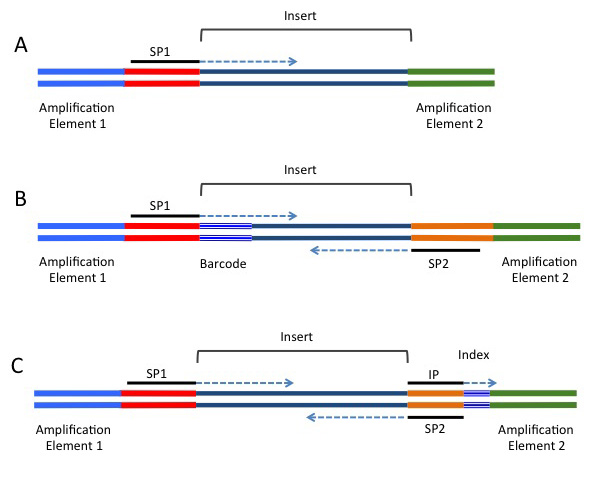
\includegraphics[width=0.7\textwidth]{images/elements.jpg}
\end{figure}
\url{http://rnaseq.uoregon.edu/}
\end{frame}


\begin{frame}{Most common problems}
\begin{itemize}
\item Firefox is unstable, so call a tutor if there's a problem
\item You can't tell the letter `\texttt{l}' from the number `\texttt{1}'
\item Long lines of code are broken by the symbol ``\textbackslash"
\item There may be a missing \~{} symbol at the start of a file path in the text  (Sorry...)
\item Always, always, always use ``Tab auto-complete"
\end{itemize}
\end{frame}

\begin{frame}{Today's Tutors}
\begin{itemize}
	\item Steve Pederson (Bioinformatics Hub, Adelaide University)
	\item Dr John Toubia (Centre For Cancer Biology)
	\item Dr Terry Bertozzi (SA Museum)
\end{itemize}
\end{frame}


\begin{frame}{Login for External Attendees}
WiFi Network: UofA \\
user: bioinfhub \\
pass: u\$hs7oaigs

\end{frame}

\end{document}